% Results
The results of the raining process are presented in this chapter. We begin by first solving outlining the training network architecture and training process on simulated XANES in section \ref{sec:nn-sim-data}. Then, we discuss the work on expanding the model to make solid predictions on experimental data.

\section{Training with Simulation Data} \label{sec:nn-sim-data}
The 1000 simulated XANES spectra were first loaded into a Pandas dataframe \cite{pandas-1} \cite{pandas-2} of shape $ 1000\times82 $. Each of the 82 columns represents a discrete energy value, and each row represents the absorption for a given spectrum at those energies. The dataset was split into training and testing groups according to an 80-20 random split, respectively. All absorption columns were then scaled via the standard scalar (\ref{z-score}) and the training labels scaled via a min-max scaler (\ref{eqn:min-max-scaler}). First, the model was trained to predict four descriptors: the mean-squared-displacement (MSD), the mean bond length distance, the standard deviation of the bond length distributions, and the skew of the bond length distribution. Note that the standard deviation is the same as the square root of the MSD. This feature was only included preliminarily in order to better understand the correlation in the network's predictions. 

\begin{figure}
    \centering
    \includegraphics[width=\linewidth]{Chapters/Figures/nn_rdf_validation_preds.png}
    \caption{One configuration of the trained neural network includes four output nodes: MSD, Sigma, Mean, and Kurtosis. Sigma is just the square root of the MSD and was included during training to affirm the patterns recognized by the network.}
    \label{fig:train-test-split-all4}
\end{figure}

\section{Experimental Data} \label{ch:results}
Training the neural network entirely on simulation data and then making predictions on experimental data is unlikely to provide quality results. Using the trained network from Table (...) that predicted the test set values in Figure \ref{fig:train-test-split-all4}, we predicted the MSD values from two experimental spectra. On the unpublished IMASC data, the netork predicted an MSD of $0.0003724~\AA^2$ instead of the EXAFS equation fitted value of ${\sigma^2=0.0102(8)~\AA^2}$. This poor prediction suggests the network considers the experimental spectrum to look most similar to the lowest disorder FEFF spectra; the model is not generalizing to understand the disorder encoded in the spectral shape.


\begin{figure}
    \centering
    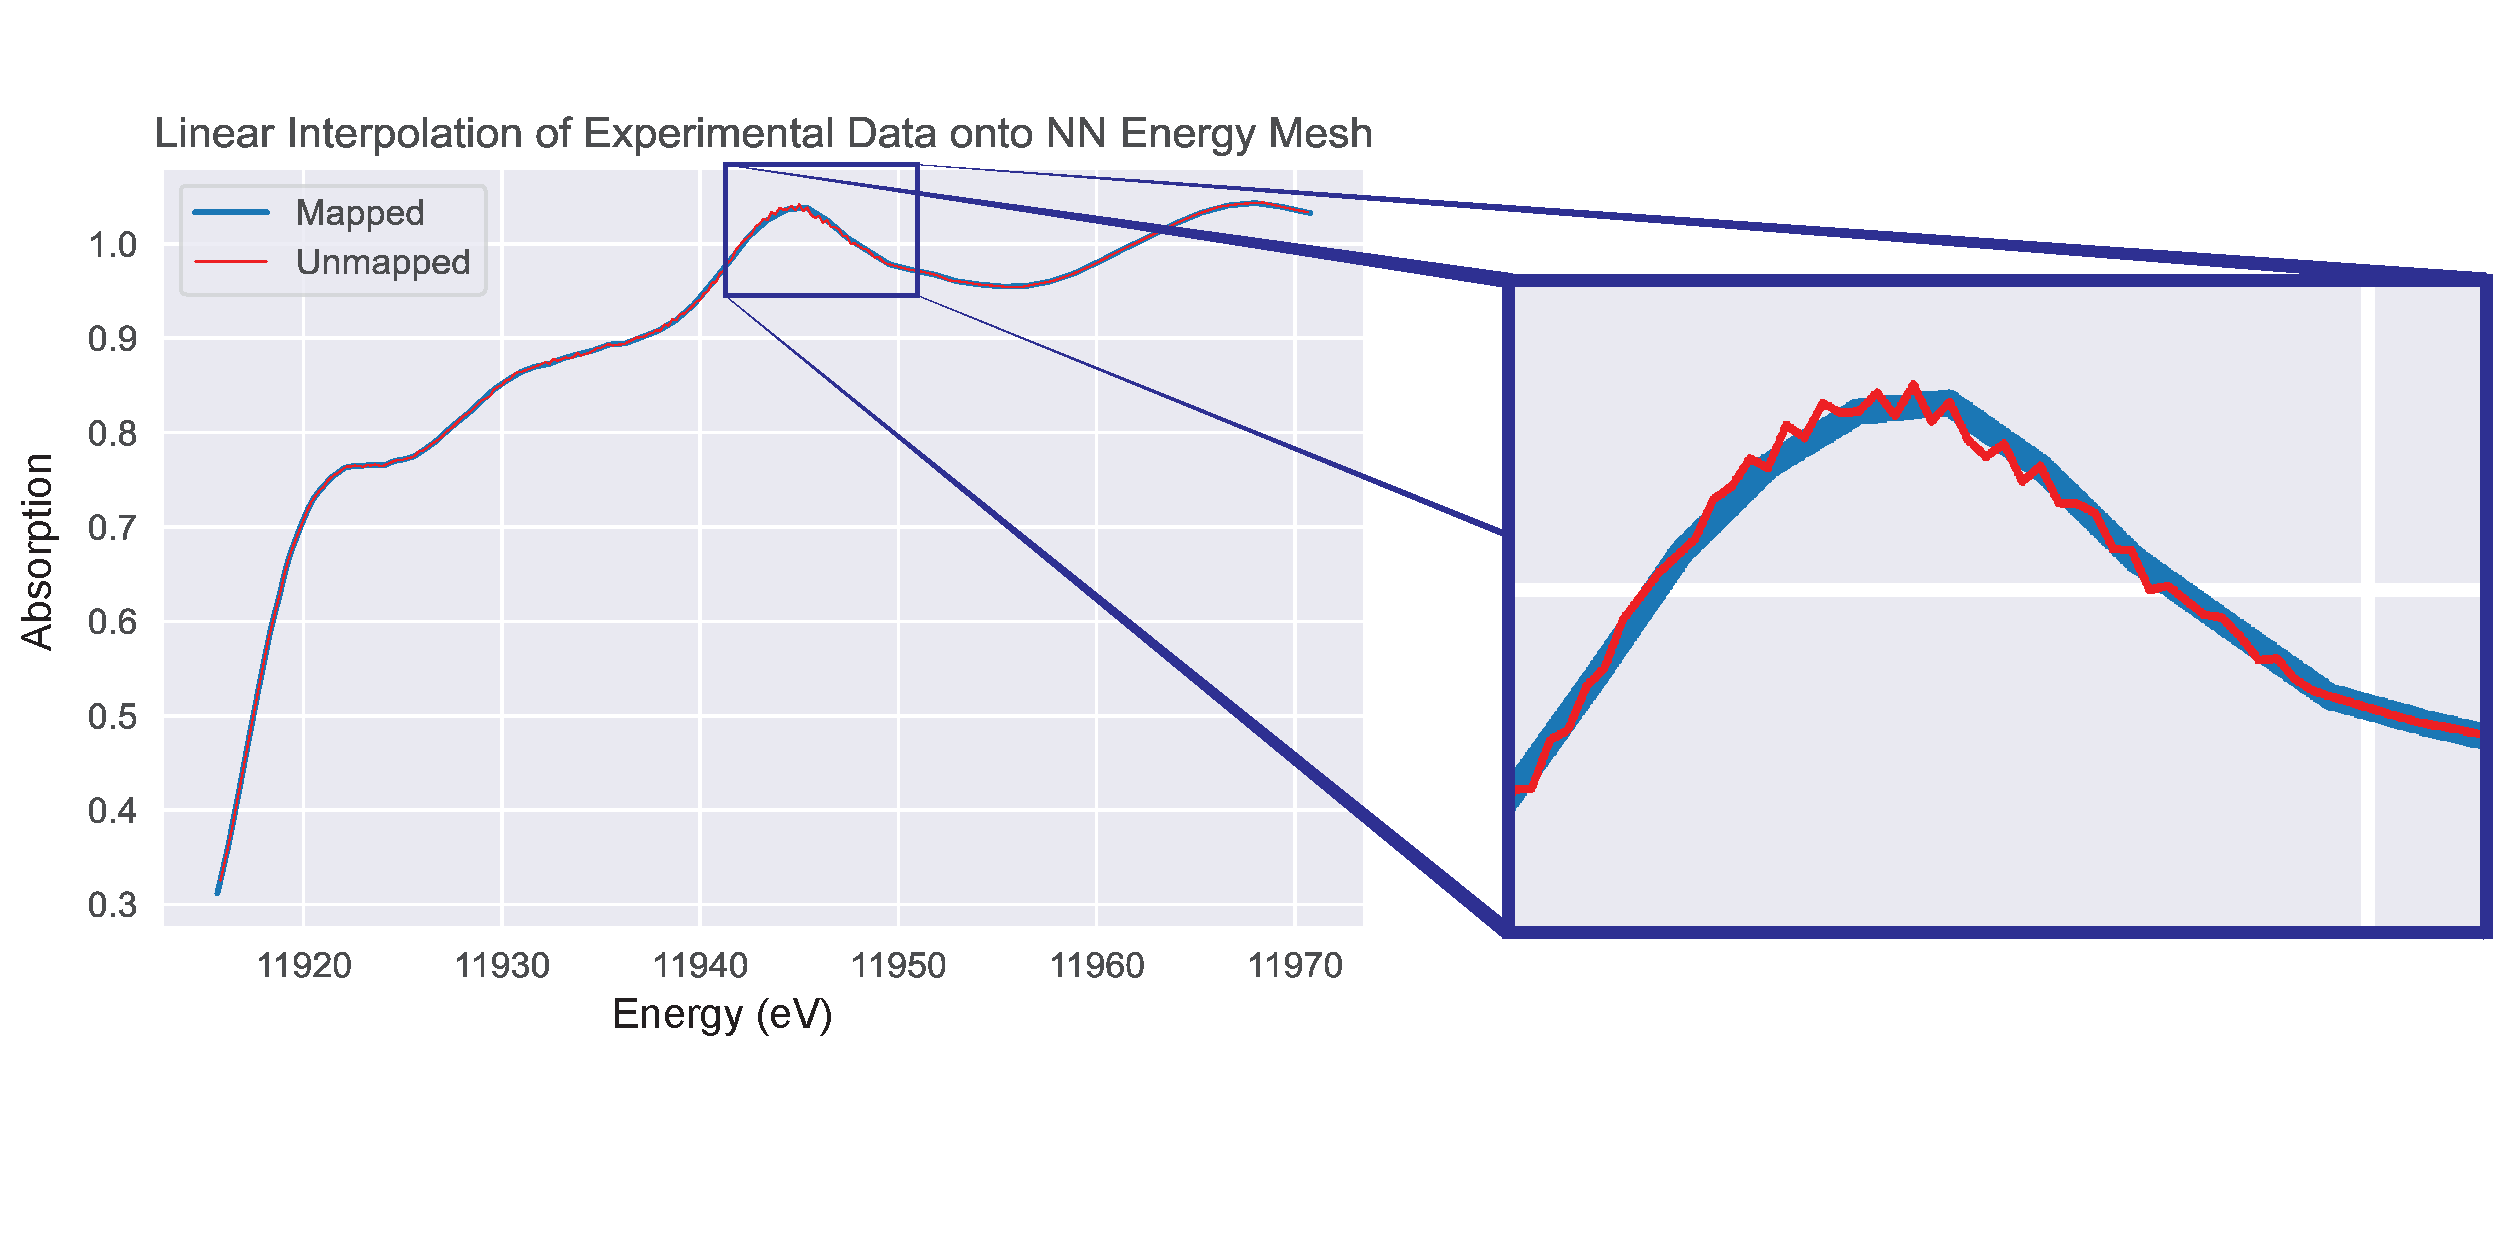
\includegraphics[width=\linewidth]{Chapters/Figures/quality-of-interpolation-skinny.pdf}
    \caption[Experimental Data Interpolation]{The experimental data is measured as a function of different energy values than the ones on which the neural network is trained. Consequently, the experimental spectrum must be mapped onto the proper energy mesh via linear interpolation.}
    \label{fig:interpolation-skinny}
\end{figure}

\subsection{Data Augmentation}
While there is ample data for training and predicting on only simulation data, we only have two experimental spectra. In order to create more training and testing data for the neural network, two types of data augmentation were utilized: horizontal spectral shifting and Gaussian noise inclusion. While the motivation for utilizing data augmentation is to expand the size of the experimental training and testing set, the neural network must be trained to recognize the augmentation types prior to training or testing on the experimental data. As such, both the FEFF simulated dataset and experimental dataset are augmented.

Noise is artificially injected into the spectra by randomly shifting each absorption coefficient vertically. The shifted value for each energy level is selected from a Gaussian distribution with standard deviation $ \sigma=0.01 $. An exaggerated example of the injected noise is shown in Figure \ref{fig:data-aug-gauss-noise}.

\begin{figure}
    \centering
    \includegraphics[width=\linewidth]{Chapters/Figures/gaussian-noise-data-aug.pdf}
    \caption[Data Augmentation: Gaussian Noise]{Gaussian noise is added to the spectra to increase the variance of the training data. This helps the network to learn the low-level features of the spectra and ignore artifacts not caused by the structural disorder. For demonstration purposes, the scale of the noise in this figure has been increased beyond what was used in training.}
    \label{fig:data-aug-gauss-noise}
\end{figure}

The second form of data augmentation is added through horizontal shifts. While this is common for signal processing and time series analysis, the inclusion here is more controversial. In XAFS, the edge location is dependent on the oxidation/reduction state of the species. Shifting the horizontal location is akin to shifting the species of the model; however, the neural network is not being tasked to determine the oxidation state of the sample. Instead, the model is only tasked with predicting the mean-squared-displacement of the nanoparticle's bond lengths. The theory is that the disorder information is encoded in the  


\begin{figure}
    \centering
    \includegraphics[width=\linewidth]{Chapters/Figures/data-aug-shift-pt75wieght.pdf}
    \caption[Data Augmentation: Horizontal Shift]{...}
    \label{fig:data-aug-hor}
\end{figure}

